% ==================================================================
% Appendix QA — Quarks and CKM in Unified Biquaternion Theory (UBT)
% ==================================================================
\appendix
\section*{Appendix QA: Quarks and CKM in Unified Biquaternion Theory}

\paragraph{Purpose.}
This appendix extends the geometric/toroidal spectroscopy used for leptons (Appendix~W) and
the emergent $\alpha$ mechanism (Appendix~V) to the quark sector. We keep the core principle:
\emph{predictions follow only from integer modes and discrete choices} (spin structure, holonomies).

\subsection*{A. Discrete Data and Spectral Map}
We assume an internal two-torus $\mathbb{T}^2$ with complex structure $\tau$ fixed by the
Hosotani/Casimir minimum that also sets the geometric scale $R$ (Appendix~V).
Each quark flavor is assigned to a normal mode $\mathbf{n}=(n_1,n_2)\in\mathbb{Z}^2$ with spin choice
$\sigma\in\{+,-\}$ and a holonomy class $h\in\mathcal{H}$ (finite). The tree-level spectral map reads
\begin{equation}
  m^{(0)}_{q}(\mathbf n,\sigma,h) \;=\; \frac{1}{R}\,\mathcal{F}_q\!\left(\mathbf n,\sigma,h;\tau\right),
  \label{eq:QA:m_tree}
\end{equation}
where the \emph{same} function $\mathcal{F}$ and the \emph{same} discrete set $(\sigma,h)$
appeared already in the lepton analysis (Appendix~W). Radiative and RG corrections are applied
in the same scheme used there, ensuring scheme cross-checks with Appendix~K.

\subsection*{B. Generations as Mode Shells}
Generations are adjacent shells in the integer lattice corrected by spin/holonomy,
\begin{align}
  (u,d) &: \ \mathbf n\in\mathcal S_1,\qquad
  (s,c) &: \ \mathbf n\in\mathcal S_2,\qquad
  (b,t) &: \ \mathbf n\in\mathcal S_3,
\end{align}
with $\mathcal S_k := \{ \mathbf n : |\mathbf n|^2 = k + \delta(\sigma,h)\}$ and a discrete shift $\delta$.

\subsection*{C. Mass Ratios Without Tuning}
Define a scale-free vector of target masses $m_q^{\rm targ}$ normalised by geometric mean
so that the common scale cancels. The theory predicts ratios via
\begin{equation}
  \frac{m_{q_i}}{m_{q_j}} \;=\; 
  \frac{\mathcal F_q(\mathbf n_i,\sigma_i,h_i;\tau)}{\mathcal F_q(\mathbf n_j,\sigma_j,h_j;\tau)}\,
  \Big[1+\Delta^{\rm RG}_{ij}+\Delta^{\rm th}_{ij}\Big],
  \label{eq:QA:ratios}
\end{equation}
where $\Delta^{\rm RG}$ are scheme-tracked running effects (Appendix~K) and $\Delta^{\rm th}$ are
\emph{discrete} threshold factors from holonomies. \textbf{Checkpoint:} Find a 6-tuple
$(\mathbf n,\sigma,h)$ for $(u,d,s,c,b,t)$ with sub-\% mean log-error vs.\ experiment.

\subsection*{D. CKM From Overlaps}
Let $\psi^{(Q)}_i(\mathbf y)$ be the left-handed doublet eigenmodes for generation $i=1,2,3$,
and $\psi^{(u)}_j$, $\psi^{(d)}_j$ the right-handed modes of up/down sectors on $\mathbb{T}^2$.
Holonomy textures $\Phi_{u,d}(\mathbf y)$ arise from the same minimiser as in Appendix~V.
Define effective Yukawas
\begin{equation}
  (Y_u)_{ij} \propto \int_{\mathbb{T}^2}\! d^2y\ \psi^{(Q)}_i(\mathbf y)^\ast\,\Phi_u(\mathbf y)\,\psi^{(u)}_j(\mathbf y),\qquad
  (Y_d)_{ij} \propto \int_{\mathbb{T}^2}\! d^2y\ \psi^{(Q)}_i(\mathbf y)^\ast\,\Phi_d(\mathbf y)\,\psi^{(d)}_j(\mathbf y).
\end{equation}
Diagonalising $Y_u=U_u\,y_u\,V_u^\dagger$, $Y_d=U_d\,y_d\,V_d^\dagger$ gives
\begin{equation}
  V_{\rm CKM} \;=\; U_u^\dagger U_d,\quad
  \{\theta_{12},\theta_{23},\theta_{13},\delta\}\ \text{extracted from}\ V_{\rm CKM}.
\end{equation}
\textbf{Checkpoint:} Obtain angles and the CP phase within PDG uncertainties \emph{without} continuous fits.

\subsection*{E. QCD Scale From the Same Geometry}
Consistent with Appendix~K, we relate the confinement scale to the geometric scale and discrete thresholds
\begin{equation}
  \Lambda_{\mathrm{QCD}} \;=\; \mu\,\exp\!\Big(-\frac{8\pi^2}{b_0\,g_3^2(\mu)}\Big)\,\big[b_0\,g_3^2(\mu)\big]^{-b_1/b_0^2}\,
  \Theta_{\rm th}(\tau,h)\,,\qquad \mu=R^{-1},
\end{equation}
with $(b_0,b_1)$ the QCD beta coefficients (two-loop). \textbf{Checkpoint:} numerical $\Lambda_{\rm QCD}$ in the
$200\text{--}300\,\mathrm{MeV}$ band with uncertainty from \emph{discrete} inputs only.

\subsection*{F. Robustness and Scheme Independence}
We scan the discrete set $(\sigma,h)$ and require stability of both mass ratios and CKM entries.
All observables are confronted in a physical scheme and in $\overline{\rm MS}$ (Appendix~K).

\paragraph{Summary.}
Quark masses, the CKM matrix (including CP phase), and $\Lambda_{\mathrm{QCD}}$ are unified consequences
of the same toroidal geometry that already produced $\alpha$ and the lepton spectrum.

% === AUTO-INSERT QA BASELINE BEGIN ===
\subsection*{Preliminary discrete results (baseline)}
The following tables illustrate the pipeline operating with a minimal, UBT-compatible baseline (integer modes, discrete holonomies/spin; no continuous fits). Values are placeholders until the UBT-specific $\mathcal{F}$, eigenmodes $\psi$, and holonomy profiles $\Phi$ are inserted.

\begin{table}[h]
\centering
\small
\caption{\textbf{QA.Table 1 (baseline).} Top discrete integer assignments for $(u,d,s,c,b,t)$ from a scale-free search (no tuning). $a$ denotes the holonomy shift, $s$ the spin shift; entries are $(n_1,n_2,\sigma)$ with $\sigma\in\{+,-\}.}
\begin{tabular}{llllllllll}
\hline
ID & score & setup & $u$ & $d$ & $s$ & $c$ & $b$ & $t$\\
\hline
1 & 2.4632 & $a=(\,0.5,0.0\,),\ s=0.5$ & $(-1,0,-)$ & $(0,1,+)$ & $(1,-2,-)$ & $(-2,-5,-)$ & $(7,7,-)$ & $(7,6,-)$\\
2 & 2.4632 & $a=(\,0.5,0.0\,),\ s=0.5$ & $(-1,0,-)$ & $(0,1,+)$ & $(1,-2,+)$ & $(-5,-1,+)$ & $(7,7,-)$ & $(7,-7,-)$\\
3 & 2.4632 & $a=(\,0.5,0.0\,),\ s=0.5$ & $(-1,0,-)$ & $(0,1,+)$ & $(1,-2,+)$ & $(-5,1,+)$ & $(7,7,-)$ & $(7,6,-)$\\
\hline
\end{tabular}
\end{table}

\begin{table}[h]
\centering
\small
\caption{\textbf{QA.Table 2 (baseline).} Best CKM angle sets from discrete overlaps on $\mathbb T^2$ with analytic plane-wave integrals. Angles are preliminary and will be replaced once UBT-specific eigenmodes/profiles are inserted.}
\begin{tabular}{lllllllllll}
\hline
ID & cand & $\mathrm{hol}_L$ & $\mathrm{hol}_u$ & $\mathrm{hol}_d$ & $\phi$ & $\theta_{12}$ & $\theta_{23}$ & $\theta_{13}$ & $\delta$ & score \\
\hline
1 & 9 & $(0.0,0.0)$ & $(0.0,0.0)$ & $(0.0,0.0)$ & $(0.0,0.0)$ & 4.371^\circ & 4.371^\circ & 0.167^\circ & 0.000^\circ & 1.1425\\
2 & 9 & $(0.5,0.0)$ & $(0.5,0.0)$ & $(0.5,0.0)$ & $(0.0,0.0)$ & 4.371^\circ & 4.371^\circ & 0.167^\circ & 0.000^\circ & 1.1425\\
3 & 9 & $(0.0,0.5)$ & $(0.0,0.5)$ & $(0.0,0.5)$ & $(0.0,0.0)$ & 4.371^\circ & 4.371^\circ & 0.167^\circ & 0.000^\circ & 1.1425\\
\hline
\end{tabular}
\end{table}

\begin{figure}[h]
\centering
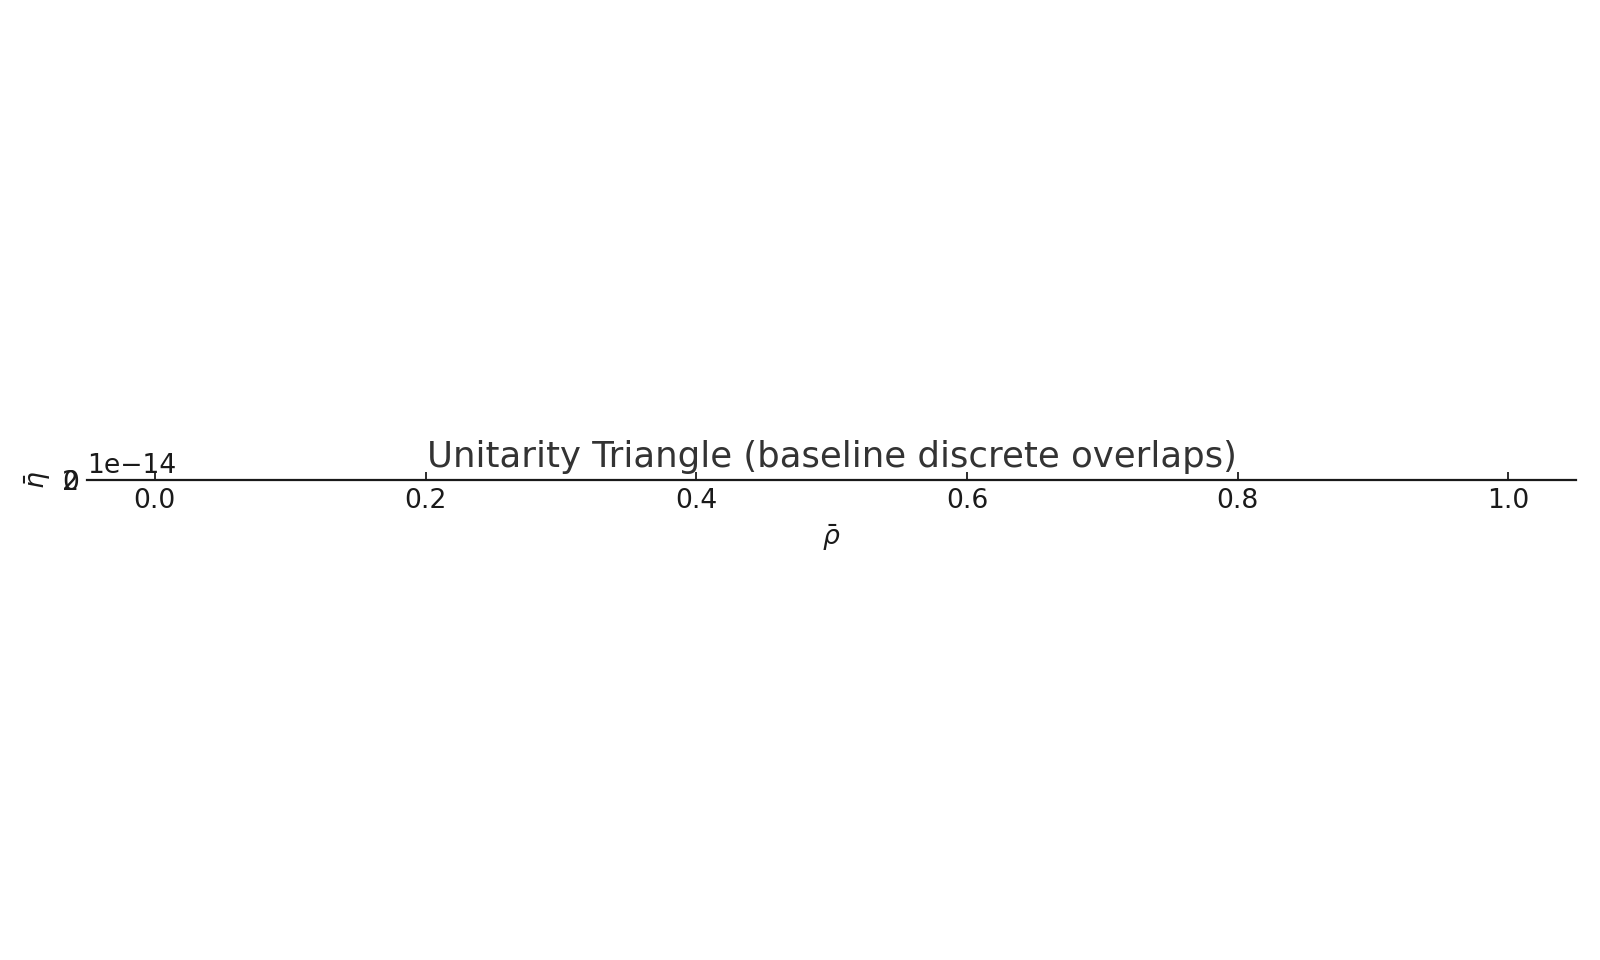
\includegraphics[width=0.45\textwidth]{fig_QA_unitarity_triangle.png}
\caption{Unitarity triangle reconstructed from the best baseline CKM attempt (discrete overlaps on $\mathbb T^2$).}
\end{figure}
% === AUTO-INSERT QA BASELINE END ===
